\section{Analys i tre dimensioner}

\paragraph{Spänning}
Vi definierar spänningsvektorn
\begin{align*}
	\vb{s} = \lim\limits_{A \to 0}\frac{\vb{F}}{A}
\end{align*}
där $\vb{F}$ är kraften på det lilla arealementet. Den har en komponent normalt på ytan, som är normalspänningen, och en komponent som är parallel med ytan, som är skjuvspänningen. Vi får
\begin{align*}
	\sigma = \vb{s}\cdot\vb{n}, \tau^{2} = \abs{\vb{s}}^{2} - \sigma^{2}.
\end{align*}

\paragraph{Skjuvspänningar i tre dimensioner}
Snitta nu ut en infinitesimal kub. På ytorna, till exempel ytan som är normal på $x$-axeln, kan man dekomponera spänningsvektorn i en normalspänning $\sigma_{x}$ och två skjuvspänningar $\tau_{xy}, \tau_{xz}$, och motsvarande i andra riktningar. Om vi tittar på momentjämvikt kring kubens centrum i $x$-riktning fås
\begin{align*}
	2\tau_{yz}\dd{x}\dd{z}\cdot\frac{1}{2}\dd{y} - 2\tau_{zy}\dd{x}\dd{y}\cdot\frac{1}{2}\dd{z}        &= 0, \\
	\tau_{yz} &= \tau_{zy}.
\end{align*}
En motsvarande härledning kan göras för de andra sidorna. Tillkommer det andra termer om skjuvspänningen varierar? Ja, men dessa kommer vara av högre ordning, och kan försummas.

\paragraph{Spänningsmatris}
Vi kan nu definiera en spänningsmatris
\begin{align*}
	S =
	\mqty[
		\sigma_{x} & \tau_{yx}  & \tau_{zx} \\
		\tau_{xy}  & \sigma_{y} & \tau_{zy} \\
		\tau_{xz}  & \tau_{yz}  & \sigma_{z}
	].
\end{align*}
Enligt argumentet ovan är denna symmetrisk.

\paragraph{Spänningar på godtycklig yta}
Om man har en godtycklig yta med normalvektor $\vb{n}$, kan det visas att spänningarna på ytan ges av
\begin{align*}
	\vb{s} = S\vb{n}.
\end{align*}
Vi kan då skriva
\begin{align*}
	\sigma &= \vb{n}^{T}S\vb{n}, \\
	\tau   &= \abs{S\vb{n}}^{2} - (\vb{n}^{T}S\vb{n})^{2}.
\end{align*}

\paragraph{Huvudspänningar}
Finns det orienteringar sådana att $\vb{s} = \sigma\vb{n}$? Att hitta sådana är ett egenvärdesproblem. Matematiken ger att det finns sådana orienteringar, och att de är ortogonala mot varandra.

Beteckna även den största respektiva minsta huvudspänningen som $\sigma_{1}$ respektiva $\sigma_{3}$. Då ges den maximala skjuvspänningen i materialet av
\begin{align*}
	\tau_{\text{max}} = \frac{\sigma_{1} - \sigma_{3}}{2}.
\end{align*}

\paragraph{Plana tillstånd}
Ett specialfall är när $z$-riktningen är en huvudriktning för spänningen. Då är skjuvspänningarna i $xy$-planet, dvs. $\tau_{zx} = \tau_{zy} = 0$. Om $\sigma_{z} = 0$, har man plan spänning.

Betrakta plan spänning på ett plan som bildar en vinkel $\phi$ med $y$-axeln. Normalvektorn ges av
\begin{align*}
	\vb{n} = \cos{\phi}\vb{e}_{x} + \sin{\phi}\vb{e}_{y}.
\end{align*}
Vi får då
\begin{align*}
	\sigma &= \sigma_{x}\cos[2]{\phi} + \sigma_{y}\sin[2]{\phi} + 2\tau_{xy}\sin{\phi}\cos{\phi}, \\
	\tau   &= \tau_{xy}\cos{2\phi} + \frac{\sigma_{y} - \sigma_{x}}{2}\sin{2\phi}.
\end{align*}

\paragraph{Mohrs spänningscirkel}
Mohrs spänningscirkel är ett sätt att grafiskt ta fram plana spänningar vid rotation av ett plan. För att konstruera cirkeln, rita upp ett $\sigma, \tau$-koordinatsystem och två punkter $(sigma_{x}, \tau_{x, y})$ och $(sigma_{y}, -\tau_{x, y})$, där dessa tas från något givet tillstånd. Dessa punkter skall vara i motstående änder av cirkeln, och från detta kan cirkeln ritas, som i figur \ref{fig:mohr_stress_circle}.

\begin{figure}[!ht]
	\centering
	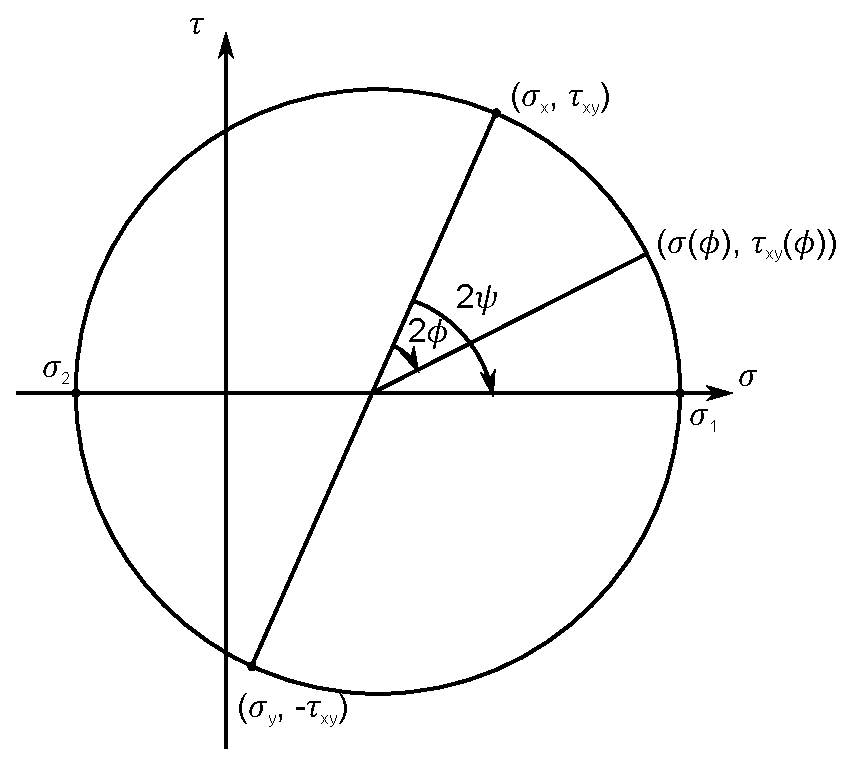
\includegraphics[width = 0.5\textwidth]{./Images/mohr_stress_circle.eps}
	\caption{Mohrs spänningscirkel.}
	\label{fig:mohr_stress_circle}
\end{figure}

En rotation moturs av koordinatsystemet med en vinkel $\phi$ motsvarar en rotation medurs av tillståndet på cirkeln med en vinkel $2\phi$.

Det visar sig att cirkeln skär $\sigma$-axeln i största och minsta huvudspänningen. Det finns även en vinkel $\psi$ som koordinatsystemet måste roteras med så att det blir parallellt med huvudriktningarna. Ur denna geometrin kan vi få följande samband, som är helt konsekventa med tensorbetraktningen gjort ovan:
\begin{align*}
	\sigma_{1}        &= \frac{\sigma_{x} + \sigma_{y}}{2} + \sqrt{\left(\frac{\sigma_{x} - \sigma_{y}}{2}\right)^{2} + \tau_{xy}^{2}}, \\
	\sigma_{2}        &= \frac{\sigma_{x} + \sigma_{y}}{2} - \sqrt{\left(\frac{\sigma_{x} - \sigma_{y}}{2}\right)^{2} + \tau_{xy}^{2}}, \\
	\tan(2\psi)       &= \frac{2\tau_{xy}}{\sigma_{x} - \sigma_{y}}, \\
	\tau_{\text{max}} &= \frac{\sigma_{1} - \sigma_{3}}{2}.
\end{align*}

\paragraph{Jämvikt i tre dimensioner}
Snitta ut en liten kub. Jämvikt i $x$-riktning ger
\begin{align*}
	\sigma(\vb{x} + \dd{x}\vb{e}_{x})\dd{y}\dd{z} - \sigma(\vb{x})\dd{y}\dd{z} + \tau_{zx}(\vb{x} + \dd{z}\vb{e}_{z})\dd{x}\dd{y} - \tau_{zx}(\vb{x})\dd{x}\dd{y} + \tau_{yx}(\vb{x} + \dd{y}\vb{e}_{y})\dd{x}\dd{z} - \tau_{yx}(\vb{x})\dd{x}\dd{z} = 0,
\end{align*}
vilket implicerar
\begin{align*}
	\del{x}{\sigma_{x}} + \del{y}{\tau_{xy}} + \del{z}{\tau_{zx}} = 0.
\end{align*}
På motsvarande sätt fås
\begin{align*}
	\del{x}{\tau_{xy}} + \del{y}{\sigma_{y}} + \del{z}{\tau_{yz}} &= 0, \\
	\del{y}{\tau_{xz}} + \del{y}{\tau_{yz}} + \del{z}{\sigma_{z}} &= 0.
\end{align*}
Om det finns volymkrafter i kroppen, dyker den även upp som en term här.

\paragraph{Töjning i tre dimensioner}
I tre dimensioner definieras töjningen i termer av båglängden som
\begin{align*}
	\varepsilon = \frac{\dd{s} - \dd{s_{0}}}{\dd{s_{0}}},
\end{align*}
där $\dd{s_{0}}$ är den odeformerade båglängden och $\dd{s}$ är den deformerade båglängden.

\paragraph{Tredimensionellt samband mellan töjning och deformation}
Betrakta en kropp som deformeras med en deformationsvektor $\vb{u}$. Snitta ut en kub och titta på två hörn i positioner $x$ och $x + \dv{x}$, med övriga koordinater lika. I det odeformerade läget är avståndet mellan dessa $\dd{s_{0}} = \dd{x}$. I det deformerade läget är avståndet
\begin{align*}
	\dd{s} &= (x + \dd{x} + u_{x}(x + \dd{x}, y, z)) - (x + u_{x}(x, y, z)) \\
	       &= \dd{x} + u_{x}(x + \dd{x}, y, z) - u_{x}(x, y, z) \\
	       &= \dd{x} + \dv{u_{x}}{x}\dd{x},
\end{align*}
och töjningen i $x$-riktning ges av
\begin{align*}
	\varepsilon_{x} = \del{x}{u_{x}}.
\end{align*}
På samma sätt fås
\begin{align*}
	\varepsilon_{y} = \del{y}{u_{y}}, \varepsilon_{z} = \del{z}{u_{z}}.
\end{align*}

\paragraph{Skjuvdeformation i tre dimensioner}
Betrakta en kub som deformeras i $xy$-planet. Sidan närmast $x$-axeln bildar vinkeln $\beta$ med $x$-axeln och sidan närmast $y$-axeln bildar vinkeln $\alpha$ med $y$-axeln. Den totala skjuvvinkeln ges av $\gamma_{yx} = \alpha + \beta$. Geometrin ger
\begin{align*}
	\gamma_{xy} = \frac{u_{x}(x, y + \dd{y}, z) - u_{x}(x, y, z)}{\dd{y}} + \frac{u_{y}(x + dd{x}, y, z) - u_{x}(x, y, z)}{\dd{x}} = \del{y}{u_{x}} + \del{x}{u_{y}}.
\end{align*}
på motsvarande sätt fås
\begin{align*}
	\gamma_{yz} = \del{z}{u_{y}} + \del{y}{u_{z}}, \gamma_{xz} = \del{z}{u_{x}} + \del{x}{u_{z}}.
\end{align*}

\paragraph{Töjningsmatrisen}
Vi definierar töjningsmatrisen
\begin{align*}
	T =
	\mqty[
		\varepsilon_{x}  & \varepsilon_{yx} & \varepsilon_{zx} \\
		\varepsilon_{xy} & \varepsilon_{y}  & \varepsilon_{zy} \\
		\varepsilon_{xz} & \varepsilon_{yz} & \varepsilon_{z}
	],
\end{align*}
där vi inför $\varepsilon_{xy} = \varepsilon_{yx} = \frac{1}{2}\gamma_{xy}$. Detta medför att $T$ är symmetrisk. Det gäller att töjningen i riktningen $\vb{n}$ ges av
\begin{align*}
	\varepsilon_{\vb{n}} = \vb{n}^{T}T\vb{n}.
\end{align*}

\paragraph{Huvudtöjningar}
Finns det orienteringar sådana att $T\vb{n} = \varepsilon\vb{n}$? Att hitta sådana är ett egenvärdesproblem. Matematiken ger att det finns sådana orienteringar, och att de är ortogonala mot varandra.

Beteckna även den största respektiva näst största huvudtöjningen som $\varepsilon_{1}$ respektiva $\varepsilon_{2}$. Då ges den maximala skjuvvinkeln i materialet av
\begin{align*}
	\gamma_{\text{max}} = \varepsilon_{1} - \varepsilon_{2}.
\end{align*}

\paragraph{Mohrs töjningscirkel}
Mohrs töjningscirkel är ett sätt att grafiskt ta fram plana töjningar vid rotation av ett plan. För att konstruera cirkeln, rita upp ett $\varepsilon, \frac{\gamma}{2}$-koordinatsystem och två punkter $(\varepsilon_{x}, \frac{\gamma_{x, y}}{2})$ och $(\varepsilon_{y}, -\frac{\gamma_{x, y}}{2})$, där dessa tas från något givet tillstånd. Dessa punkter skall vara i motstående änder av cirkeln, och från detta kan cirkeln ritas, som i figur \ref{fig:mohr_strain_circle}.

\begin{figure}[!ht]
	\centering
	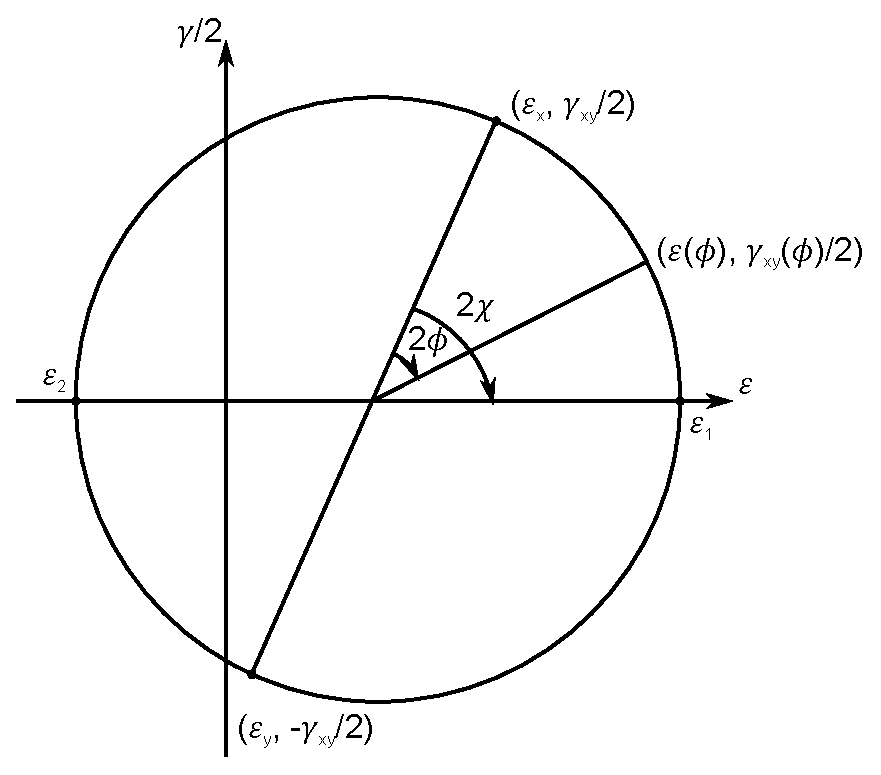
\includegraphics[width = 0.5\textwidth]{./Images/mohr_strain_circle.eps}
	\caption{Mohrs töjningscirkel.}
	\label{fig:mohr_strain_circle}
\end{figure}

En rotation moturs av planet med en vinkel $\phi$ motsvarar en rotation medurs av tillståndet på cirkeln med en vinkel $2\phi$.

Det visar sig att cirkeln skär $\varepsilon$-axeln i största och näst största huvudtöjningen. Det finns även en vinkel $\chi$ som koordinatsystemet måste roteras med så att det blir parallellt med huvudriktningarna. Ur denna geometrin kan vi få följande samband, som är helt konsekventa med tensorbetraktningen gjort ovan:
\begin{align*}
	\varepsilon_{1}     &= \frac{\varepsilon_{x} + \varepsilon_{y}}{2} + \sqrt{\left(\frac{\varepsilon_{x} - \varepsilon_{y}}{2}\right)^{2} + \left(\frac{\gamma_{xy}}{2}\right)^{2}}, \\
	\varepsilon_{2}     &= \frac{\varepsilon_{x} + \varepsilon_{y}}{2} - \sqrt{\left(\frac{\varepsilon_{x} - \varepsilon_{y}}{2}\right)^{2} + \left(\frac{\gamma_{xy}}{2}\right)^{2}}, \\
	\tan(2\psi)         &= \frac{\gamma_{xy}}{\varepsilon_{x} - \varepsilon_{y}}, \\
	\gamma_{\text{max}} &= \varepsilon_{1} - \varepsilon_{2}.
\end{align*}

\paragraph{Kompatibilitet i tre dimensioner}
Från definitionerna av elementerna i töjningsmatrisen kan man se att det gäller att
\begin{align*}
	2\del{x}{\del{y}{\varepsilon_{xy}}} &= \del[2]{y}{\varepsilon_{x}} + \del[2]{x}{\varepsilon_{y}}, \\
	2\del{y}{\del{z}{\varepsilon_{yz}}} &= \del[2]{z}{\varepsilon_{y}} + \del[2]{y}{\varepsilon_{z}}, \\
	2\del{z}{\del{x}{\varepsilon_{zx}}} &= \del[2]{x}{\varepsilon_{z}} + \del[2]{z}{\varepsilon_{x}}.
\end{align*}
Alltså är inte de olika töjningarna oberoende.

\paragraph{Linjärelastiska material}
I linjärelastiska material gäller sambandet $S = CT$, där $C$ är en fjärde ordningens tensor. Detta kan alternativt skrivas som $T = C^{-1}S$.

\paragraph{Hookes lag för isotropa material}
I isotropa material är alla riktningar lika. I dessa materialer gäller Hookes lag
\begin{align*}
	\varepsilon_{x} &= \frac{1}{E}(\sigma_{x} - \nu(\sigma_{y} + \sigma_{z})) + \alpha\Delta T, \\
	\varepsilon_{y} &= \frac{1}{E}(\sigma_{y} - \nu(\sigma_{x} + \sigma_{z})) + \alpha\Delta T, \\
	\varepsilon_{z} &= \frac{1}{E}(\sigma_{z} - \nu(\sigma_{x} + \sigma_{y})) + \alpha\Delta T, \\
	\gamma_{xy}     &= \frac{1}{G}\tau_{xy}, \\
	\gamma_{yz}     &= \frac{1}{G}\tau_{yz}, \\
	\gamma_{xz}     &= \frac{1}{G}\tau_{xz},
\end{align*}
där $E$ är elasticitetsmodulen, $G$ är skjuvmodulen och $\nu$ är Poissons tal.

\paragraph{Samband mellan elasticitetsmodul och skjuvmodul}
Betrakta ett plant skjuvtillstånd med skjuvspänning $\tau_{xy}$ för ett isotropt material. Med Moores spänningscirkel fås huvudspänningarna $\sigma_{1} = \tau_{xy}, \sigma_{2} = -\tau_{xy}$. Hookes lag ger
\begin{align*}
	\varepsilon_{1} = \frac{1 + \nu}{E}\tau_{xy}, \varepsilon_{2} = -\frac{1 + \nu}{E}\tau_{xy}.
\end{align*}
Mohrs töjningscirkel ger vidare
\begin{align*}
	\frac{\gamma_{xy}}{2} = \varepsilon_{1} = \frac{1 + \nu}{E}\tau_{xy}.
\end{align*}
Jämförelse med Hookes lag ger
\begin{align*}
	G = \frac{1}{2(1 + \nu)}E.
\end{align*}